\documentclass[aspectratio=169,10pt]{beamer}

\usetheme{default}
\usecolortheme{default}
\setbeamertemplate{navigation symbols}{}
\setbeamertemplate{footline}[frame number]
\setbeamertemplate{itemize item}{\textbullet}
\setbeamertemplate{itemize subitem}{\textendash}

\definecolor{LaidlawNavy}{HTML}{1B2A41}
\definecolor{LaidlawTeal}{HTML}{3D6B6E}
\definecolor{LaidlawRust}{HTML}{A85A3A}
\definecolor{LaidlawGray}{HTML}{E8EAED}
\definecolor{LaidlawText}{HTML}{2C2C2C}
\definecolor{LaidlawSoft}{HTML}{F4F6F8}

\setbeamercolor{normal text}{fg=LaidlawText,bg=white}
\setbeamercolor{structure}{fg=LaidlawTeal}
\setbeamercolor{title}{fg=LaidlawNavy}
\setbeamercolor{frametitle}{fg=LaidlawNavy}
\setbeamerfont{frametitle}{series=\bfseries,size=\large}

\usepackage{amssymb}
\usepackage{array}
\usepackage{booktabs}
\usepackage{graphicx}
\usepackage{microtype}
\usepackage{tabularx}
\usepackage{tikz}

\setlength{\leftmargini}{1.15em}
\setlength{\itemsep}{0.28em}
\renewcommand{\arraystretch}{1.12}
\newcolumntype{Y}{>{\raggedright\arraybackslash}X}

\newcommand{\callout}[1]{%
  \begin{tikzpicture}
    \node[
      fill=LaidlawSoft,
      draw=LaidlawGray,
      rounded corners=2pt,
      inner xsep=8pt,
      inner ysep=5pt,
      text width=0.92\textwidth,
      align=left,
      font=\footnotesize
    ] {#1};
  \end{tikzpicture}%
}

\begin{document}

%----------------------------------------------------------------------
\begin{frame}[plain]
  \vspace{1.85cm}
  {\color{LaidlawNavy}\LARGE\bfseries Weather definitions with Hogan\par}

  \vspace{1.45em}
  {\normalsize Bob\par}
  \vspace{0.25em}
  {\normalsize 28 July 2026\par}
\end{frame}

%----------------------------------------------------------------------
\begin{frame}{Listen first}
  \begin{columns}[T]
    \begin{column}{0.47\textwidth}
      {\color{LaidlawTeal}\large\textbf{Hogan frames the question}}
      \begin{itemize}
        \item How do you see the weather question now?
        \item What would make the later-period comparison useful?
        \item What should we simplify, correct, or protect?
      \end{itemize}
    \end{column}
    \begin{column}{0.49\textwidth}
      {\color{LaidlawTeal}\large\textbf{Bob listens and writes}}
      \begin{itemize}
        \item Put genuine choices on the table
        \item Record Hogan's wording
        \item Read it back before leaving
      \end{itemize}
    \end{column}
  \end{columns}

  \vspace{0.65em}
  \callout{\textbf{Credit.} Li et al.\ provide the \emph{Atmospheric Research}
  heatwave event family. Hogan proposed the project adaptation:
  count events by month, then identify upper-tail months.
  Hogan leads the weather framing.}
\end{frame}

%----------------------------------------------------------------------
\begin{frame}{One named family; different estimands}
  \footnotesize
  \begin{tabularx}{\textwidth}{@{}>{\bfseries\color{LaidlawNavy}}p{0.20\textwidth}Y@{}}
    \toprule
    Jasmine confirmed &
    Liu J et al.\ (2020): Hong Kong daily mortality.
    Reported attributable fractions were \textbf{4.72\% for cold}
    and \textbf{0.16\% for heat}. \\
    \addlinespace
    Roro's siblings &
    \texttt{HWD\_Tavg}, \texttt{HWD\_Tmax},
    \texttt{HWD\_Tmin}, and \texttt{HWD\_Tcombined}.
    Keep all four as distinct named candidates. \\
    \addlinespace
    Current project &
    Monthly thermal exposures paired with true-event-month stroke
    aggregates, subject to Roro's governed outcome rules. \\
    \bottomrule
  \end{tabularx}

  \vspace{0.7em}
  \callout{The evidence is cumulative, not interchangeable.
  Tuesday chooses exposure definitions before any project health results are inspected.}
\end{frame}

%----------------------------------------------------------------------
\begin{frame}{Heat and cold coexist across the study window}
  \begin{center}
    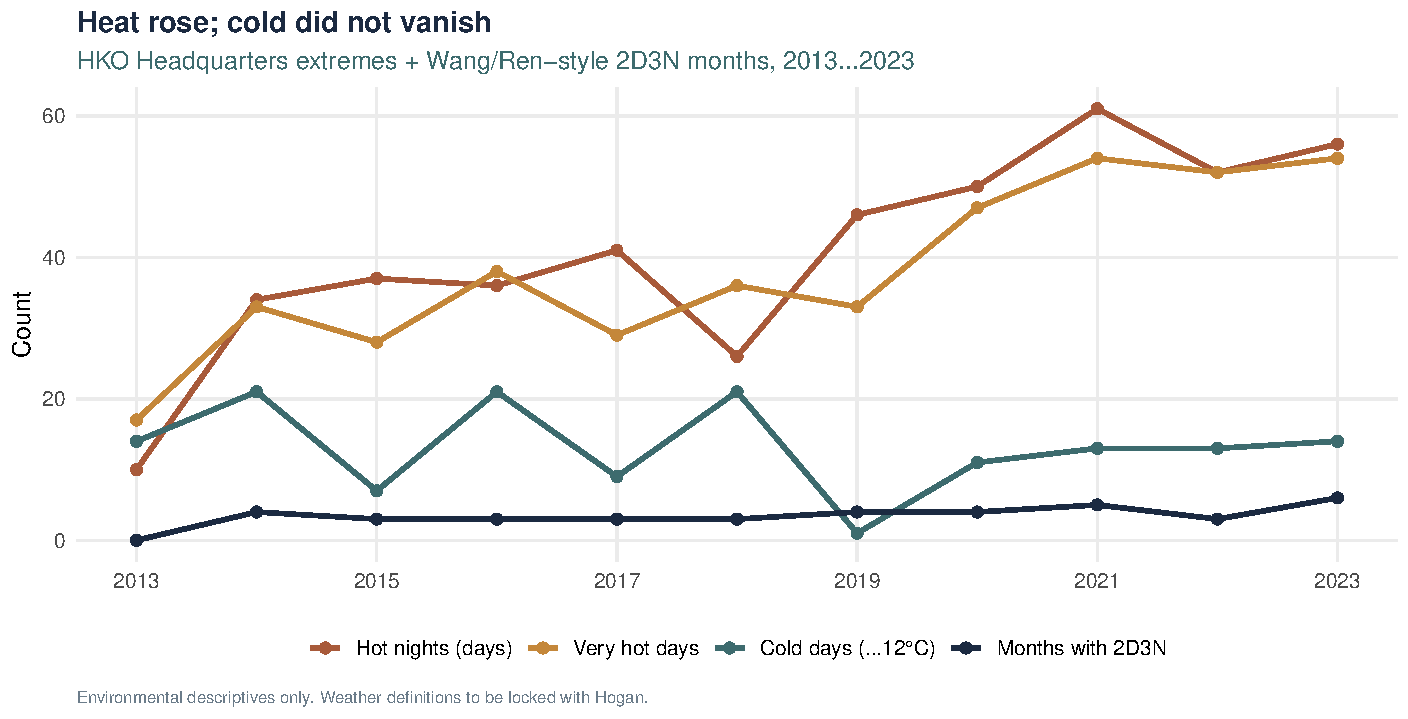
\includegraphics[width=0.88\textwidth,height=0.72\textheight,keepaspectratio]
      {../../figures/hogan_tuesday/fig_annual_coexistence.pdf}
  \end{center}
  \vspace{-0.35em}
  \begin{center}
    \scriptsize Exposure-only description for discussion with Hogan; no stroke findings.
  \end{center}
\end{frame}

%----------------------------------------------------------------------
\begin{frame}{Relative tails depend on the reference freeze}
  \begin{center}
    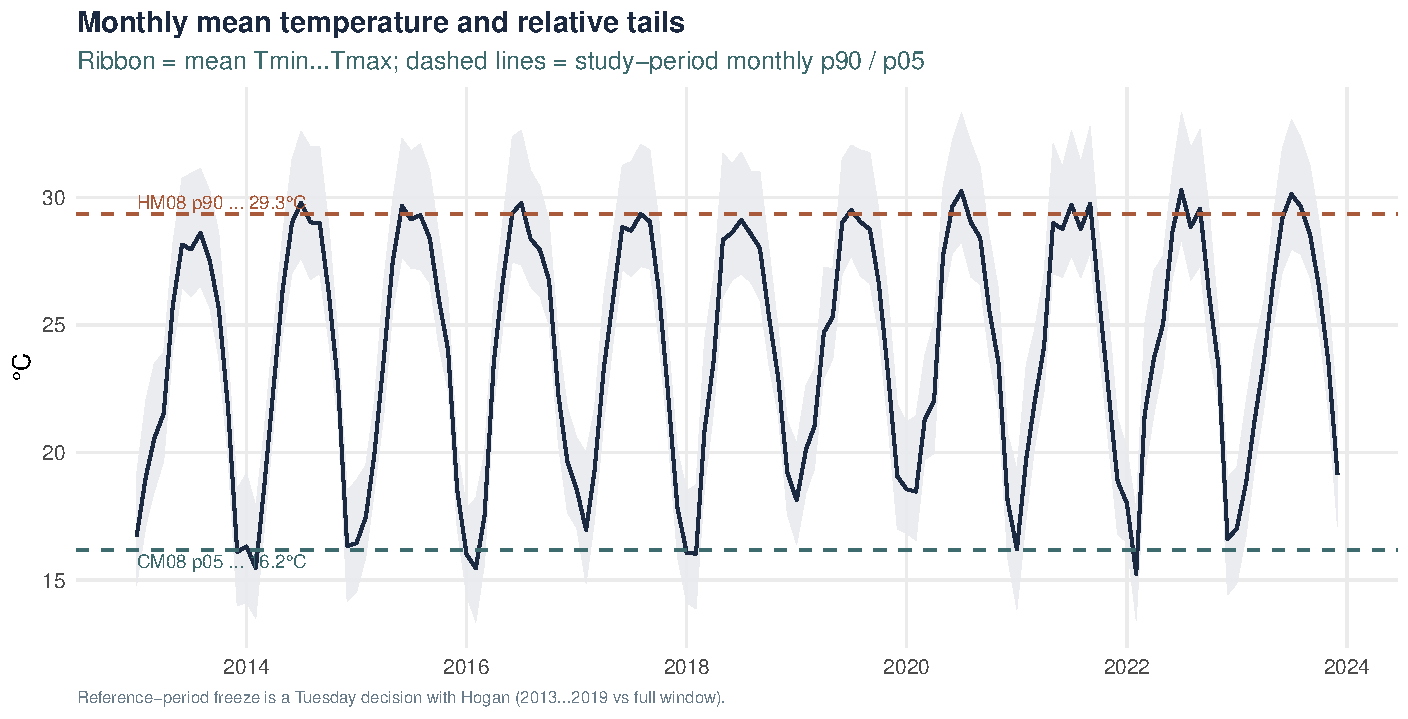
\includegraphics[width=0.88\textwidth,height=0.72\textheight,keepaspectratio]
      {../../figures/hogan_tuesday/fig_monthly_temp_tails.pdf}
  \end{center}
  \vspace{-0.35em}
  \begin{center}
    \scriptsize Decision needed: 2013--2019, full 2013--2023, or a defensible external climatology?
  \end{center}
\end{frame}

%----------------------------------------------------------------------
\begin{frame}{Prevalence is a design check, not a winner}
  \begin{center}
    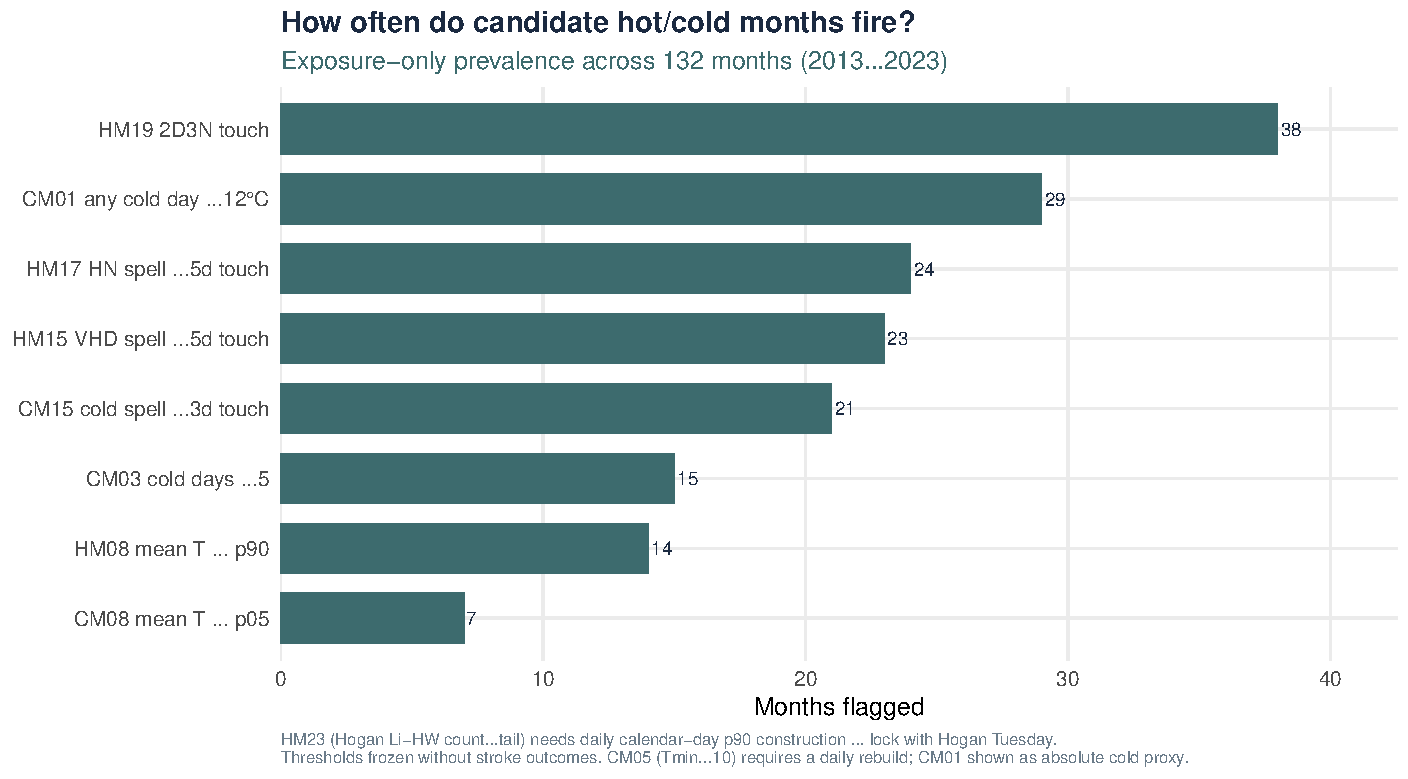
\includegraphics[width=0.88\textwidth,height=0.72\textheight,keepaspectratio]
      {../../figures/hogan_tuesday/fig_starter_prevalence.pdf}
  \end{center}
  \vspace{-0.35em}
  \begin{center}
    \scriptsize Counts help test usability. They do not choose a definition by themselves.
  \end{center}
\end{frame}

%----------------------------------------------------------------------
\begin{frame}{Starter hot-month and cold-month set}
  \scriptsize
  \begin{tabularx}{\textwidth}{@{}>{\bfseries\color{LaidlawRust}}p{0.08\textwidth}Y
    >{\bfseries\color{LaidlawTeal}}p{0.08\textwidth}Y@{}}
    \toprule
    \multicolumn{2}{c}{\color{LaidlawRust}\textbf{Hot-month starters}} &
    \multicolumn{2}{c}{\color{LaidlawTeal}\textbf{Cold-month starters}} \\
    \midrule
    HM23 & Li-HW event-count upper tail; lock with Hogan &
    CM03 & At least five days with \(T_{\min}\leq12^\circ\)C \\
    HM08 & Monthly mean temperature at or above frozen p90 &
    CM08 & Monthly mean temperature at or below frozen p05 \\
    HM15 & Touches at least five consecutive \(T_{\max}\geq33^\circ\)C days &
    CM15 & Touches at least three consecutive \(T_{\min}\leq12^\circ\)C days \\
    HM17 & Touches at least five consecutive \(T_{\min}\geq28^\circ\)C nights &
    & \\
    HM19 & Touches a Wang/Ren-style 2D3N window &
    & \\
    \bottomrule
  \end{tabularx}

  \vspace{0.55em}
  \callout{\textbf{First-wave sensitivities:}
  HM27 nighttime heat-degree burden; HM32 heat + ozone;
  CM05 any \(T_{\min}\leq10^\circ\)C day; CM30 cold + influenza.
  CM05 stays a labelled severe-cold sensitivity, not biology.}
\end{frame}

%----------------------------------------------------------------------
\begin{frame}{Six decisions to lock together}
  \footnotesize
  \begin{columns}[T]
    \begin{column}{0.49\textwidth}
      \(\square\) \textbf{Li-HW / HM23}\\
      Season, p90 operator, duration, gaps, monthly assignment, and tie rule.

      \vspace{0.75em}
      \(\square\) \textbf{Gate 3 pair}\\
      Name one hot and one cold co-primary.

      \vspace{0.75em}
      \(\square\) \textbf{Roro siblings}\\
      Place all four \texttt{HWD\_*} definitions in the named family?
    \end{column}
    \begin{column}{0.49\textwidth}
      \(\square\) \textbf{Reference freeze}\\
      Choose the primary threshold period and percentile method.

      \vspace{0.75em}
      \(\square\) \textbf{CM05 role}\\
      Keep it as severe-cold sensitivity only?

      \vspace{0.75em}
      \(\square\) \textbf{Age visibility}\\
      Retain 65--69 and 70--74 if governance permits?
    \end{column}
  \end{columns}

  \vspace{0.75em}
  \callout{Write each decision in Hogan's words. If something stays open,
  record the precise question, owner, and date.}
\end{frame}

%----------------------------------------------------------------------
\begin{frame}[plain]
  \vspace{1.15cm}
  {\color{LaidlawNavy}\LARGE\bfseries Thank you, Hogan\par}

  \vspace{0.75em}
  {\large\color{LaidlawTeal}For leading the weather side and helping make it clearer.\par}

  \vspace{1.0em}
  \begin{itemize}
    \item Read back the six written decisions
    \item Correct the wording together
    \item Send the short record to Hogan and Roro
  \end{itemize}

  \vspace{0.9em}
  {\small No rush on anything that needs a little more thought :)\par}
\end{frame}

\end{document}
